% Options for packages loaded elsewhere
\PassOptionsToPackage{unicode}{hyperref}
\PassOptionsToPackage{hyphens}{url}
%
\documentclass[
]{article}
\usepackage{amsmath,amssymb}
\usepackage{iftex}
\ifPDFTeX
  \usepackage[T1]{fontenc}
  \usepackage[utf8]{inputenc}
  \usepackage{textcomp} % provide euro and other symbols
\else % if luatex or xetex
  \usepackage{unicode-math} % this also loads fontspec
  \defaultfontfeatures{Scale=MatchLowercase}
  \defaultfontfeatures[\rmfamily]{Ligatures=TeX,Scale=1}
\fi
\usepackage{lmodern}
\ifPDFTeX\else
  % xetex/luatex font selection
\fi
% Use upquote if available, for straight quotes in verbatim environments
\IfFileExists{upquote.sty}{\usepackage{upquote}}{}
\IfFileExists{microtype.sty}{% use microtype if available
  \usepackage[]{microtype}
  \UseMicrotypeSet[protrusion]{basicmath} % disable protrusion for tt fonts
}{}
\makeatletter
\@ifundefined{KOMAClassName}{% if non-KOMA class
  \IfFileExists{parskip.sty}{%
    \usepackage{parskip}
  }{% else
    \setlength{\parindent}{0pt}
    \setlength{\parskip}{6pt plus 2pt minus 1pt}}
}{% if KOMA class
  \KOMAoptions{parskip=half}}
\makeatother
\usepackage{xcolor}
\usepackage[margin=1in]{geometry}
\usepackage{color}
\usepackage{fancyvrb}
\newcommand{\VerbBar}{|}
\newcommand{\VERB}{\Verb[commandchars=\\\{\}]}
\DefineVerbatimEnvironment{Highlighting}{Verbatim}{commandchars=\\\{\}}
% Add ',fontsize=\small' for more characters per line
\usepackage{framed}
\definecolor{shadecolor}{RGB}{248,248,248}
\newenvironment{Shaded}{\begin{snugshade}}{\end{snugshade}}
\newcommand{\AlertTok}[1]{\textcolor[rgb]{0.94,0.16,0.16}{#1}}
\newcommand{\AnnotationTok}[1]{\textcolor[rgb]{0.56,0.35,0.01}{\textbf{\textit{#1}}}}
\newcommand{\AttributeTok}[1]{\textcolor[rgb]{0.13,0.29,0.53}{#1}}
\newcommand{\BaseNTok}[1]{\textcolor[rgb]{0.00,0.00,0.81}{#1}}
\newcommand{\BuiltInTok}[1]{#1}
\newcommand{\CharTok}[1]{\textcolor[rgb]{0.31,0.60,0.02}{#1}}
\newcommand{\CommentTok}[1]{\textcolor[rgb]{0.56,0.35,0.01}{\textit{#1}}}
\newcommand{\CommentVarTok}[1]{\textcolor[rgb]{0.56,0.35,0.01}{\textbf{\textit{#1}}}}
\newcommand{\ConstantTok}[1]{\textcolor[rgb]{0.56,0.35,0.01}{#1}}
\newcommand{\ControlFlowTok}[1]{\textcolor[rgb]{0.13,0.29,0.53}{\textbf{#1}}}
\newcommand{\DataTypeTok}[1]{\textcolor[rgb]{0.13,0.29,0.53}{#1}}
\newcommand{\DecValTok}[1]{\textcolor[rgb]{0.00,0.00,0.81}{#1}}
\newcommand{\DocumentationTok}[1]{\textcolor[rgb]{0.56,0.35,0.01}{\textbf{\textit{#1}}}}
\newcommand{\ErrorTok}[1]{\textcolor[rgb]{0.64,0.00,0.00}{\textbf{#1}}}
\newcommand{\ExtensionTok}[1]{#1}
\newcommand{\FloatTok}[1]{\textcolor[rgb]{0.00,0.00,0.81}{#1}}
\newcommand{\FunctionTok}[1]{\textcolor[rgb]{0.13,0.29,0.53}{\textbf{#1}}}
\newcommand{\ImportTok}[1]{#1}
\newcommand{\InformationTok}[1]{\textcolor[rgb]{0.56,0.35,0.01}{\textbf{\textit{#1}}}}
\newcommand{\KeywordTok}[1]{\textcolor[rgb]{0.13,0.29,0.53}{\textbf{#1}}}
\newcommand{\NormalTok}[1]{#1}
\newcommand{\OperatorTok}[1]{\textcolor[rgb]{0.81,0.36,0.00}{\textbf{#1}}}
\newcommand{\OtherTok}[1]{\textcolor[rgb]{0.56,0.35,0.01}{#1}}
\newcommand{\PreprocessorTok}[1]{\textcolor[rgb]{0.56,0.35,0.01}{\textit{#1}}}
\newcommand{\RegionMarkerTok}[1]{#1}
\newcommand{\SpecialCharTok}[1]{\textcolor[rgb]{0.81,0.36,0.00}{\textbf{#1}}}
\newcommand{\SpecialStringTok}[1]{\textcolor[rgb]{0.31,0.60,0.02}{#1}}
\newcommand{\StringTok}[1]{\textcolor[rgb]{0.31,0.60,0.02}{#1}}
\newcommand{\VariableTok}[1]{\textcolor[rgb]{0.00,0.00,0.00}{#1}}
\newcommand{\VerbatimStringTok}[1]{\textcolor[rgb]{0.31,0.60,0.02}{#1}}
\newcommand{\WarningTok}[1]{\textcolor[rgb]{0.56,0.35,0.01}{\textbf{\textit{#1}}}}
\usepackage{graphicx}
\makeatletter
\def\maxwidth{\ifdim\Gin@nat@width>\linewidth\linewidth\else\Gin@nat@width\fi}
\def\maxheight{\ifdim\Gin@nat@height>\textheight\textheight\else\Gin@nat@height\fi}
\makeatother
% Scale images if necessary, so that they will not overflow the page
% margins by default, and it is still possible to overwrite the defaults
% using explicit options in \includegraphics[width, height, ...]{}
\setkeys{Gin}{width=\maxwidth,height=\maxheight,keepaspectratio}
% Set default figure placement to htbp
\makeatletter
\def\fps@figure{htbp}
\makeatother
\setlength{\emergencystretch}{3em} % prevent overfull lines
\providecommand{\tightlist}{%
  \setlength{\itemsep}{0pt}\setlength{\parskip}{0pt}}
\setcounter{secnumdepth}{-\maxdimen} % remove section numbering
\ifLuaTeX
  \usepackage{selnolig}  % disable illegal ligatures
\fi
\IfFileExists{bookmark.sty}{\usepackage{bookmark}}{\usepackage{hyperref}}
\IfFileExists{xurl.sty}{\usepackage{xurl}}{} % add URL line breaks if available
\urlstyle{same}
\hypersetup{
  pdftitle={R Notebook},
  hidelinks,
  pdfcreator={LaTeX via pandoc}}

\title{R Notebook}
\author{}
\date{\vspace{-2.5em}}

\begin{document}
\maketitle

\hypertarget{business-requirements}{%
\subsection{Business requirements}\label{business-requirements}}

In the report I am hoping to find out more about the incidence of cancer
in NHS Borders. The Key Perfomance Indicators I will be looking at are
the number of new cases(incidences) recorded between 1997 - 2022 and see
if there are any relationships related to demographics of the NHS
Borders population.

\hypertarget{data-used}{%
\subsection{Data used}\label{data-used}}

Data for this report came from NHS open data published on
\url{https://www.opendata.nhs.scot/}. This analysis is based on the
following reports: ``opendata\_inc1721comb\_hb'' and also
``opendata\_inc\_9721\_hb''. The data has already been cleaned and
summarised.

\hypertarget{software-and-libraries-used}{%
\subsection{Software and libraries
used}\label{software-and-libraries-used}}

The report has been created in RStudio using R 4.3.0 and tidyverse
package.

\hypertarget{additional-data-cleaning-and-wrangling}{%
\subsection{Additional data cleaning and
wrangling}\label{additional-data-cleaning-and-wrangling}}

I have selected columns from the reports that were corresponding with
the information I found crucial in order to explore KPIs. I have also
pivoted data including demographics related to age.

\begin{Shaded}
\begin{Highlighting}[]
\FunctionTok{library}\NormalTok{(tidyverse)}
\end{Highlighting}
\end{Shaded}

\begin{verbatim}
## Warning: package 'tidyverse' was built under R version 4.2.3
\end{verbatim}

\begin{verbatim}
## Warning: package 'ggplot2' was built under R version 4.2.3
\end{verbatim}

\begin{verbatim}
## Warning: package 'tibble' was built under R version 4.2.3
\end{verbatim}

\begin{verbatim}
## Warning: package 'dplyr' was built under R version 4.2.3
\end{verbatim}

\begin{verbatim}
## -- Attaching core tidyverse packages ------------------------ tidyverse 2.0.0 --
## v dplyr     1.1.2     v readr     2.1.4
## v forcats   1.0.0     v stringr   1.5.0
## v ggplot2   3.4.2     v tibble    3.2.1
## v lubridate 1.9.2     v tidyr     1.3.0
## v purrr     1.0.1     
## -- Conflicts ------------------------------------------ tidyverse_conflicts() --
## x dplyr::filter() masks stats::filter()
## x dplyr::lag()    masks stats::lag()
## i Use the ]8;;http://conflicted.r-lib.org/conflicted package]8;; to force all conflicts to become errors
\end{verbatim}

\begin{Shaded}
\begin{Highlighting}[]
\NormalTok{colour\_scheme }\OtherTok{\textless{}{-}}  \FunctionTok{c}\NormalTok{(}\StringTok{"\#E69F00"}\NormalTok{, }\StringTok{"\#56B4E9"}\NormalTok{, }\StringTok{"\#009E73"}\NormalTok{, }\StringTok{"\#F0E442"}\NormalTok{, }\StringTok{"\#0072B2"}\NormalTok{, }\StringTok{"\#D55E00"}\NormalTok{, }\StringTok{"\#CC79A7"}\NormalTok{)}
\NormalTok{cancer\_1 }\OtherTok{\textless{}{-}} \FunctionTok{read\_csv}\NormalTok{(}\StringTok{"data/opendata\_inc1721comb\_hb.csv"}\NormalTok{)}
\end{Highlighting}
\end{Shaded}

\begin{verbatim}
## Rows: 1632 Columns: 59
## -- Column specification --------------------------------------------------------
## Delimiter: ","
## chr (10): HB, CancerSiteICD10Code, CancerSite, Sex, SexQF, Year, EASRLower95...
## dbl (49): IncidencesAgeUnder5, IncidencesAge5To9, IncidencesAge10To14, Incid...
## 
## i Use `spec()` to retrieve the full column specification for this data.
## i Specify the column types or set `show_col_types = FALSE` to quiet this message.
\end{verbatim}

\begin{Shaded}
\begin{Highlighting}[]
\NormalTok{cancer\_2 }\OtherTok{\textless{}{-}} \FunctionTok{read\_csv}\NormalTok{(}\StringTok{"data/opendata\_inc9721\_hb.csv"}\NormalTok{)}
\end{Highlighting}
\end{Shaded}

\begin{verbatim}
## Rows: 47600 Columns: 23
## -- Column specification --------------------------------------------------------
## Delimiter: ","
## chr  (9): HB, CancerSiteICD10Code, CancerSite, Sex, SexQF, EASRLower95pcConf...
## dbl (14): Year, IncidencesAllAges, CrudeRate, CrudeRateLower95pcConfidenceIn...
## 
## i Use `spec()` to retrieve the full column specification for this data.
## i Specify the column types or set `show_col_types = FALSE` to quiet this message.
\end{verbatim}

\begin{Shaded}
\begin{Highlighting}[]
\NormalTok{hb }\OtherTok{\textless{}{-}} \FunctionTok{read\_csv}\NormalTok{(}\StringTok{"data/health\_board.csv"}\NormalTok{) }\SpecialCharTok{\%\textgreater{}\%} \FunctionTok{select}\NormalTok{(HB, HBName)}
\end{Highlighting}
\end{Shaded}

\begin{verbatim}
## Rows: 18 Columns: 6
## -- Column specification --------------------------------------------------------
## Delimiter: ","
## chr (3): HB, HBName, Country
## dbl (3): _id, HBDateEnacted, HBDateArchived
## 
## i Use `spec()` to retrieve the full column specification for this data.
## i Specify the column types or set `show_col_types = FALSE` to quiet this message.
\end{verbatim}

\begin{Shaded}
\begin{Highlighting}[]
\CommentTok{\# tidying up columns}
\NormalTok{cancer\_1\_short }\OtherTok{\textless{}{-}}\NormalTok{ cancer\_1 }\SpecialCharTok{\%\textgreater{}\%} \FunctionTok{select}\NormalTok{(HB, CancerSite, Sex, Year, IncidencesAgeUnder5, IncidencesAge10To14, IncidencesAge5To9, IncidencesAge15To19, IncidencesAge20To24, IncidencesAge20To24, IncidencesAge20To24, IncidencesAge25To29, IncidencesAge30To34, IncidencesAge35To39, IncidencesAge40To44, IncidencesAge45To49, IncidencesAge50To54, IncidencesAge55To59, IncidencesAge60To64, IncidencesAge65To69, IncidencesAge70To74, IncidencesAge75To79, IncidencesAge80To84, IncidencesAge85AndOver)}

\CommentTok{\# pivoting age incidences into rows}
\NormalTok{cancer\_pivot }\OtherTok{\textless{}{-}}\NormalTok{ cancer\_1\_short }\SpecialCharTok{\%\textgreater{}\%} \FunctionTok{pivot\_longer}\NormalTok{(}\AttributeTok{cols =} \FunctionTok{starts\_with}\NormalTok{(}\StringTok{"Incidences"}\NormalTok{), }\AttributeTok{names\_to =} \StringTok{"age"}\NormalTok{, }\AttributeTok{values\_to =} \StringTok{"cases\_count"}\NormalTok{)}
\CommentTok{\# removing word "Incdences from each age row}
\NormalTok{cancer\_pivot }\OtherTok{\textless{}{-}}\NormalTok{ cancer\_pivot }\SpecialCharTok{\%\textgreater{}\%} \FunctionTok{mutate}\NormalTok{(}\AttributeTok{age =} \FunctionTok{str\_remove\_all}\NormalTok{(age, }\StringTok{"Incidences"}\NormalTok{))}
\end{Highlighting}
\end{Shaded}

\begin{Shaded}
\begin{Highlighting}[]
\CommentTok{\# add HB names onto the cancer\_2}
\NormalTok{cancer\_2 }\OtherTok{\textless{}{-}} \FunctionTok{left\_join}\NormalTok{(cancer\_2, hb, }\AttributeTok{by =} \StringTok{"HB"}\NormalTok{)}
\end{Highlighting}
\end{Shaded}

\hypertarget{at-first-i-wanted-to-see-if-nhs-borders-has-lower-or-higher-cancer-incidence-rate-that-other-scottish-health-boards.}{%
\subsubsection{1. At first I wanted to see if NHS Borders has lower or
higher cancer incidence rate that other Scottish Health
Boards.}\label{at-first-i-wanted-to-see-if-nhs-borders-has-lower-or-higher-cancer-incidence-rate-that-other-scottish-health-boards.}}

\begin{Shaded}
\begin{Highlighting}[]
 \CommentTok{\# explore where NHS Borders sits in comparison to other Health Boards In terms of number of cancer Incidences}

\NormalTok{cancer\_2 }\SpecialCharTok{\%\textgreater{}\%} 
  \FunctionTok{filter}\NormalTok{(CancerSite }\SpecialCharTok{==} \StringTok{"All cancer types"} \SpecialCharTok{\&}\NormalTok{ Sex }\SpecialCharTok{!=} \StringTok{"All"} \SpecialCharTok{\&}\NormalTok{ Year }\SpecialCharTok{==} \DecValTok{2008}\NormalTok{) }\SpecialCharTok{\%\textgreater{}\%} 
  \FunctionTok{ggplot}\NormalTok{(}\FunctionTok{aes}\NormalTok{(}\AttributeTok{x =}\NormalTok{ HBName, }\AttributeTok{y =}\NormalTok{ IncidencesAllAges, }\AttributeTok{group =}\NormalTok{ Year, }\AttributeTok{fill =}\NormalTok{ HBName))}\SpecialCharTok{+}
  \FunctionTok{geom\_col}\NormalTok{()}\SpecialCharTok{+}
  \FunctionTok{theme\_minimal}\NormalTok{()}\SpecialCharTok{+}
  \FunctionTok{labs}\NormalTok{(}
    \AttributeTok{title =} \StringTok{"}\SpecialCharTok{\textbackslash{}n}\StringTok{Cancer Incidence According to Health Board}\SpecialCharTok{\textbackslash{}n}\StringTok{"}\NormalTok{,}
    \AttributeTok{x =} \StringTok{"}\SpecialCharTok{\textbackslash{}n}\StringTok{Health Board}\SpecialCharTok{\textbackslash{}n}\StringTok{"}\NormalTok{, }
    \AttributeTok{y =} \StringTok{"}\SpecialCharTok{\textbackslash{}n}\StringTok{Count}\SpecialCharTok{\textbackslash{}n}\StringTok{"}\NormalTok{)}\SpecialCharTok{+}
  \FunctionTok{theme}\NormalTok{(}
    \AttributeTok{axis.text.x =} \FunctionTok{element\_text}\NormalTok{(}\AttributeTok{angle =} \DecValTok{45}\NormalTok{, }\AttributeTok{hjust =} \DecValTok{1}\NormalTok{, }\AttributeTok{size =} \DecValTok{10}\NormalTok{),}
  \AttributeTok{axis.text.y =} \FunctionTok{element\_text}\NormalTok{(}\AttributeTok{size =} \DecValTok{14}\NormalTok{),}
    \AttributeTok{legend.position =} \StringTok{"none"}\NormalTok{,}
    \AttributeTok{title =} \FunctionTok{element\_text}\NormalTok{(}\AttributeTok{face =} \StringTok{"bold"}\NormalTok{, }\AttributeTok{size =} \DecValTok{16}\NormalTok{))}
\end{Highlighting}
\end{Shaded}

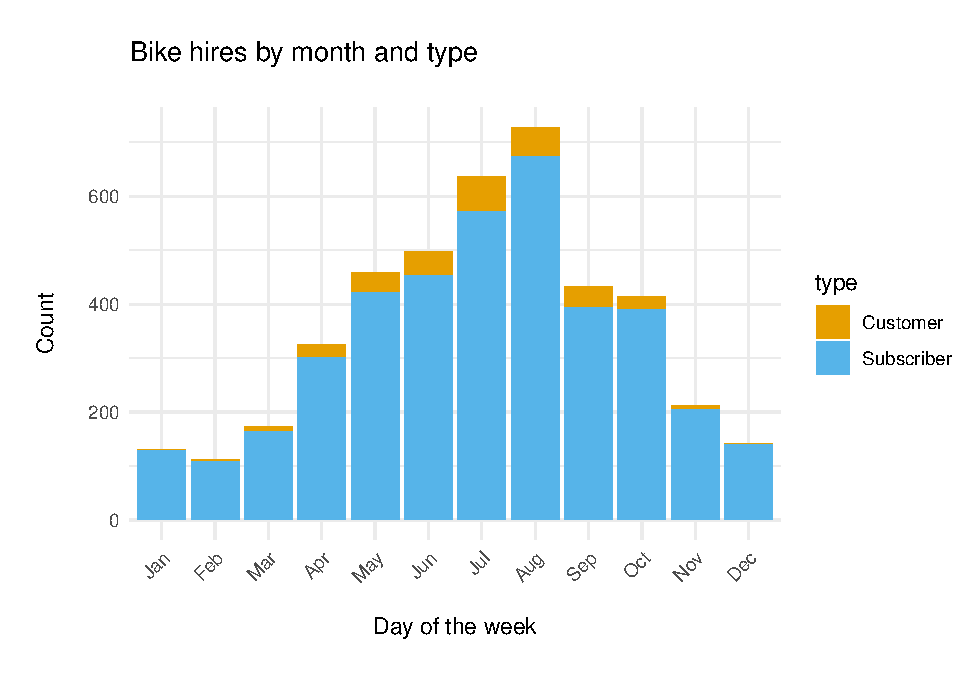
\includegraphics{report_files/figure-latex/unnamed-chunk-3-1.pdf} It
turns out that NHS Borders has 4th lowest number of new cancers recorded
- this is very likely to be linked with the size of the population
living in NHS Borders health board.

\hypertarget{then-i-checked-how-how-caner-incdence-rate-looked-over-time-for-nhs-borders.}{%
\subsubsection{2. Then I checked how how caner incdence rate looked over
time for NHS
Borders.}\label{then-i-checked-how-how-caner-incdence-rate-looked-over-time-for-nhs-borders.}}

\begin{Shaded}
\begin{Highlighting}[]
\NormalTok{cancer\_2 }\SpecialCharTok{\%\textgreater{}\%}\FunctionTok{filter}\NormalTok{(CancerSite }\SpecialCharTok{==} \StringTok{"All cancer types"} \SpecialCharTok{\&}\NormalTok{ HB }\SpecialCharTok{==} \StringTok{"S08000016"} \SpecialCharTok{\&}\NormalTok{ Sex }\SpecialCharTok{!=} \StringTok{"All"}\NormalTok{) }\SpecialCharTok{\%\textgreater{}\%} 
  \FunctionTok{ggplot}\NormalTok{(}\FunctionTok{aes}\NormalTok{(}\AttributeTok{x =}\NormalTok{ Year, }\AttributeTok{y =}\NormalTok{ IncidencesAllAges, }\AttributeTok{group =}\NormalTok{ Sex, }\AttributeTok{colour =}\NormalTok{ Sex))}\SpecialCharTok{+}
  \FunctionTok{geom\_line}\NormalTok{(}\AttributeTok{size =}\DecValTok{1}\NormalTok{)}\SpecialCharTok{+}
  \FunctionTok{scale\_x\_continuous}\NormalTok{(}\AttributeTok{breaks =} \FunctionTok{c}\NormalTok{(}\DecValTok{1997}\NormalTok{, }\DecValTok{1999}\NormalTok{, }\DecValTok{2001}\NormalTok{,}\DecValTok{2003}\NormalTok{, }\DecValTok{2005}\NormalTok{, }\DecValTok{2007}\NormalTok{, }\DecValTok{2009}\NormalTok{, }\DecValTok{2011}\NormalTok{, }\DecValTok{2013}\NormalTok{, }\DecValTok{2015}\NormalTok{, }\DecValTok{2017}\NormalTok{, }\DecValTok{2019}\NormalTok{, }\DecValTok{2021}\NormalTok{))}\SpecialCharTok{+}
   \FunctionTok{theme\_minimal}\NormalTok{()}\SpecialCharTok{+}
  \FunctionTok{labs}\NormalTok{(}
    \AttributeTok{title =} \StringTok{"}\SpecialCharTok{\textbackslash{}n}\StringTok{Cancer Incidence in NHS Borders 1997{-}2021}\SpecialCharTok{\textbackslash{}n}\StringTok{"}\NormalTok{,}
    \AttributeTok{x =} \StringTok{"}\SpecialCharTok{\textbackslash{}n}\StringTok{Year}\SpecialCharTok{\textbackslash{}n}\StringTok{"}\NormalTok{, }
    \AttributeTok{y =} \StringTok{"}\SpecialCharTok{\textbackslash{}n}\StringTok{Count}\SpecialCharTok{\textbackslash{}n}\StringTok{"}\NormalTok{)}\SpecialCharTok{+}
  \FunctionTok{theme}\NormalTok{(}
    \AttributeTok{axis.text.x =} \FunctionTok{element\_text}\NormalTok{(}\AttributeTok{angle =} \DecValTok{45}\NormalTok{, }\AttributeTok{hjust =} \DecValTok{1}\NormalTok{, }\AttributeTok{size =} \DecValTok{10}\NormalTok{),}
  \AttributeTok{axis.text.y =} \FunctionTok{element\_text}\NormalTok{(}\AttributeTok{size =} \DecValTok{14}\NormalTok{),}
    
    \AttributeTok{title =} \FunctionTok{element\_text}\NormalTok{(}\AttributeTok{face =} \StringTok{"bold"}\NormalTok{, }\AttributeTok{size =} \DecValTok{16}\NormalTok{))}
\end{Highlighting}
\end{Shaded}

\begin{verbatim}
## Warning: Using `size` aesthetic for lines was deprecated in ggplot2 3.4.0.
## i Please use `linewidth` instead.
## This warning is displayed once every 8 hours.
## Call `lifecycle::last_lifecycle_warnings()` to see where this warning was
## generated.
\end{verbatim}

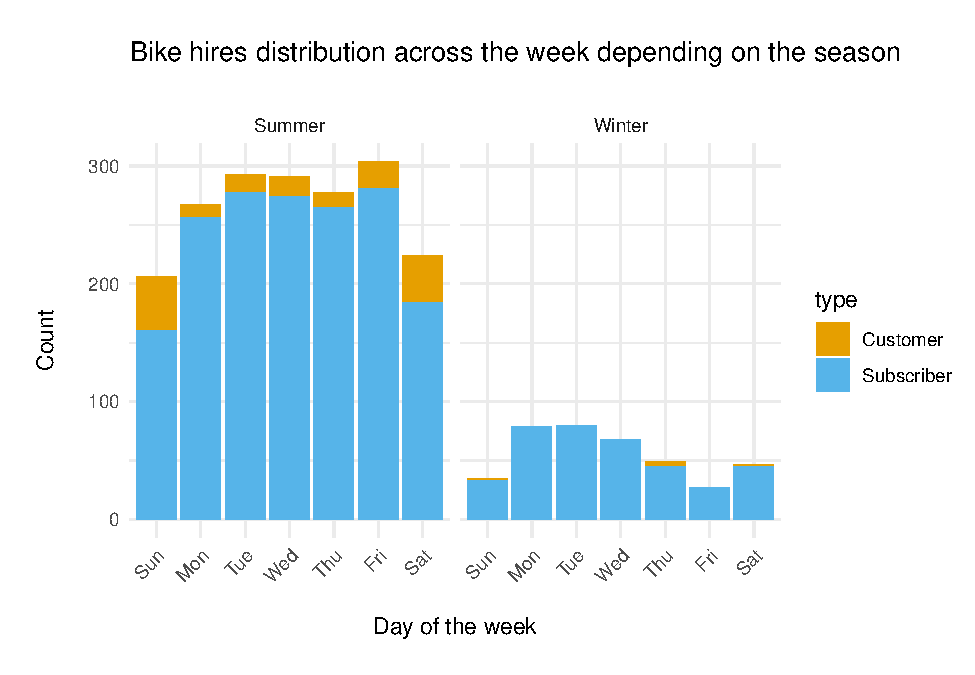
\includegraphics{report_files/figure-latex/unnamed-chunk-4-1.pdf}

We can see the rise in the number of incidences being recorded across
time, for both genders with a significant dip in 2020 for males. It is
interesting to see that teh diagnosis of cancer in females was at a
similar level between 2018 and 2020.

\hypertarget{afterwards-i-checked-what-cancer-types-were-diagnosed-more-frequently-in-nhs-borders-and-focused-only-on-those-that-had-more-than-50-cases-recorded-per-year.}{%
\subsubsection{3. Afterwards I checked what cancer types were diagnosed
more frequently in NHS Borders and focused only on those that had more
than 50 cases recorded per
year.}\label{afterwards-i-checked-what-cancer-types-were-diagnosed-more-frequently-in-nhs-borders-and-focused-only-on-those-that-had-more-than-50-cases-recorded-per-year.}}

\begin{Shaded}
\begin{Highlighting}[]
\CommentTok{\# 8 types of cancers that have been diagnosed more frequently in NHS Borders over time (at lest 50 times or more per year)}

\NormalTok{cancer\_2 }\SpecialCharTok{\%\textgreater{}\%}  
  \FunctionTok{filter}\NormalTok{(IncidencesAllAges }\SpecialCharTok{\textgreater{}=} \DecValTok{50} \SpecialCharTok{\&}\NormalTok{ HBName }\SpecialCharTok{==} \StringTok{"NHS Borders"} \SpecialCharTok{\&}\NormalTok{ CancerSite }\SpecialCharTok{!=} \StringTok{"All cancer types"} \SpecialCharTok{\&}\NormalTok{ Sex }\SpecialCharTok{!=} \StringTok{"All"}\NormalTok{) }\SpecialCharTok{\%\textgreater{}\%}
  \FunctionTok{group\_by}\NormalTok{(CancerSite) }\SpecialCharTok{\%\textgreater{}\%} \CommentTok{\#}
  \FunctionTok{ggplot}\NormalTok{(}\FunctionTok{aes}\NormalTok{(}\AttributeTok{x =}\NormalTok{ Year, }\AttributeTok{y =}\NormalTok{ IncidencesAllAges, }\AttributeTok{colour =}\NormalTok{ CancerSite))}\SpecialCharTok{+}
  \FunctionTok{geom\_line}\NormalTok{()}\SpecialCharTok{+}
  \FunctionTok{facet\_wrap}\NormalTok{(}\SpecialCharTok{\textasciitilde{}}\NormalTok{ CancerSite)}\SpecialCharTok{+}
  \FunctionTok{theme\_minimal}\NormalTok{()}\SpecialCharTok{+}
  \FunctionTok{labs}\NormalTok{(}
    \AttributeTok{title =} \StringTok{"}\SpecialCharTok{\textbackslash{}n}\StringTok{Cancers diagnosed more frequently}\SpecialCharTok{\textbackslash{}n}\StringTok{"}\NormalTok{,}
    \AttributeTok{x =} \StringTok{"}\SpecialCharTok{\textbackslash{}n}\StringTok{Year}\SpecialCharTok{\textbackslash{}n}\StringTok{"}\NormalTok{, }
    \AttributeTok{y =} \StringTok{"}\SpecialCharTok{\textbackslash{}n}\StringTok{Count}\SpecialCharTok{\textbackslash{}n}\StringTok{"}\NormalTok{)}\SpecialCharTok{+}
  \FunctionTok{theme}\NormalTok{(}
    \AttributeTok{axis.text.x =} \FunctionTok{element\_text}\NormalTok{(}\AttributeTok{angle =} \DecValTok{45}\NormalTok{, }\AttributeTok{hjust =} \DecValTok{1}\NormalTok{, }\AttributeTok{size =} \DecValTok{10}\NormalTok{),}
  \AttributeTok{axis.text.y =} \FunctionTok{element\_text}\NormalTok{(}\AttributeTok{size =} \DecValTok{10}\NormalTok{),}
    \AttributeTok{legend.position =} \StringTok{"none"}\NormalTok{,}
    \AttributeTok{title =} \FunctionTok{element\_text}\NormalTok{(}\AttributeTok{face =} \StringTok{"bold"}\NormalTok{, }\AttributeTok{size =} \DecValTok{16}\NormalTok{))}
\end{Highlighting}
\end{Shaded}

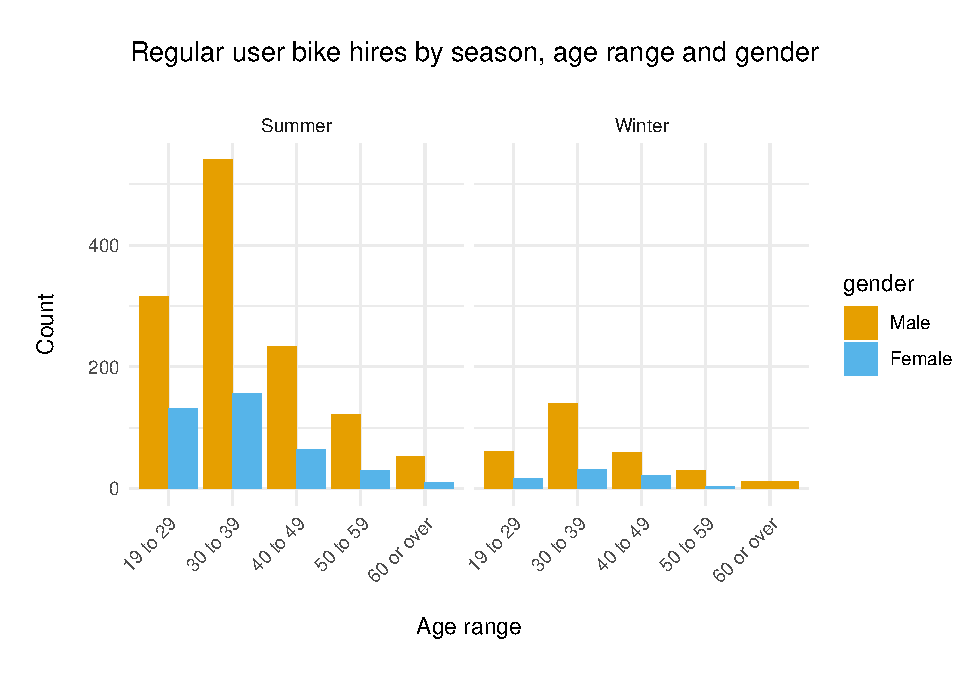
\includegraphics{report_files/figure-latex/unnamed-chunk-5-1.pdf} We can
notice that colorectal cancer, trachea, broncus and lung cancer, and
Carcinoma in situ of the cervix uteri seem to oscillate around the same
level across time, so I will focus more on those cancers that show a
growing trend in terms of number of cases over time - skin cancers,
breast and prostate cancers and explore them further.

\begin{Shaded}
\begin{Highlighting}[]
\CommentTok{\# main focus from now on will be on the past 5 years only {-} 2017{-}2022}
\NormalTok{cancer\_1\_short }\OtherTok{\textless{}{-}}\NormalTok{ cancer\_1 }\SpecialCharTok{\%\textgreater{}\%} \FunctionTok{select}\NormalTok{(HB, CancerSite, Sex, Year, IncidencesAgeUnder5, IncidencesAge10To14, IncidencesAge5To9, IncidencesAge15To19, IncidencesAge20To24, IncidencesAge20To24, IncidencesAge20To24, IncidencesAge25To29, IncidencesAge30To34, IncidencesAge35To39, IncidencesAge40To44, IncidencesAge45To49, IncidencesAge50To54, IncidencesAge55To59, IncidencesAge60To64, IncidencesAge65To69, IncidencesAge70To74, IncidencesAge75To79, IncidencesAge80To84, IncidencesAge85AndOver)}

\NormalTok{cancer\_pivot }\OtherTok{\textless{}{-}}\NormalTok{ cancer\_1\_short }\SpecialCharTok{\%\textgreater{}\%} \FunctionTok{pivot\_longer}\NormalTok{(}\AttributeTok{cols =} \FunctionTok{starts\_with}\NormalTok{(}\StringTok{"Incidences"}\NormalTok{), }\AttributeTok{names\_to =} \StringTok{"age"}\NormalTok{, }\AttributeTok{values\_to =} \StringTok{"cases\_count"}\NormalTok{)}

\NormalTok{cancer\_pivot }\OtherTok{\textless{}{-}}\NormalTok{ cancer\_pivot }\SpecialCharTok{\%\textgreater{}\%} \FunctionTok{mutate}\NormalTok{(}\AttributeTok{age =} \FunctionTok{str\_remove\_all}\NormalTok{(age, }\StringTok{"Incidences"}\NormalTok{))}
\NormalTok{cancer\_pivot}
\end{Highlighting}
\end{Shaded}

\begin{verbatim}
## # A tibble: 29,376 x 6
##    HB        CancerSite       Sex   Year      age       cases_count
##    <chr>     <chr>            <chr> <chr>     <chr>           <dbl>
##  1 S08000015 All cancer types All   2017-2021 AgeUnder5          12
##  2 S08000015 All cancer types All   2017-2021 Age10To14          11
##  3 S08000015 All cancer types All   2017-2021 Age5To9             9
##  4 S08000015 All cancer types All   2017-2021 Age15To19          29
##  5 S08000015 All cancer types All   2017-2021 Age20To24          29
##  6 S08000015 All cancer types All   2017-2021 Age25To29          58
##  7 S08000015 All cancer types All   2017-2021 Age30To34          96
##  8 S08000015 All cancer types All   2017-2021 Age35To39         156
##  9 S08000015 All cancer types All   2017-2021 Age40To44         206
## 10 S08000015 All cancer types All   2017-2021 Age45To49         363
## # i 29,366 more rows
\end{verbatim}

\begin{Shaded}
\begin{Highlighting}[]
\CommentTok{\#tidy up the age column}

\NormalTok{cancer\_pivot }\OtherTok{\textless{}{-}}\NormalTok{ cancer\_pivot }\SpecialCharTok{\%\textgreater{}\%} 
  \FunctionTok{mutate}\NormalTok{(}\AttributeTok{age =} \FunctionTok{case\_when}\NormalTok{(}
\NormalTok{    age }\SpecialCharTok{==} \StringTok{"AgeUnder5"} \SpecialCharTok{\textasciitilde{}} \StringTok{"0{-}5"}\NormalTok{,}
\NormalTok{    age }\SpecialCharTok{==} \StringTok{"Age5To9"} \SpecialCharTok{\textasciitilde{}} \StringTok{"5{-}9"}\NormalTok{,}
\NormalTok{    age }\SpecialCharTok{==} \StringTok{"Age10To14"} \SpecialCharTok{\textasciitilde{}} \StringTok{"10{-}14"}\NormalTok{,}
\NormalTok{    age }\SpecialCharTok{==} \StringTok{"Age15To19"} \SpecialCharTok{\textasciitilde{}} \StringTok{"15{-}19"}\NormalTok{, }
\NormalTok{    age }\SpecialCharTok{==} \StringTok{"Age20To24"} \SpecialCharTok{\textasciitilde{}} \StringTok{"20{-}24"}\NormalTok{,}
\NormalTok{    age }\SpecialCharTok{==} \StringTok{"Age25To29"} \SpecialCharTok{\textasciitilde{}} \StringTok{"25{-}29"}\NormalTok{,}
\NormalTok{    age }\SpecialCharTok{==} \StringTok{"Age30To34"} \SpecialCharTok{\textasciitilde{}} \StringTok{"30{-}34"}\NormalTok{,}
\NormalTok{    age }\SpecialCharTok{==} \StringTok{"Age35To39"} \SpecialCharTok{\textasciitilde{}} \StringTok{"35{-}39"}\NormalTok{,               }
\NormalTok{    age }\SpecialCharTok{==} \StringTok{"Age40To44"} \SpecialCharTok{\textasciitilde{}} \StringTok{"40{-}44"}\NormalTok{,       }
\NormalTok{    age }\SpecialCharTok{==} \StringTok{"Age45To49"} \SpecialCharTok{\textasciitilde{}} \StringTok{"45{-}49"}\NormalTok{,}
\NormalTok{    age }\SpecialCharTok{==} \StringTok{"Age50To54"} \SpecialCharTok{\textasciitilde{}} \StringTok{"50{-}54"}\NormalTok{,               }
\NormalTok{      age }\SpecialCharTok{==} \StringTok{"Age55To59"} \SpecialCharTok{\textasciitilde{}} \StringTok{"55{-}59"}\NormalTok{,}
\NormalTok{    age }\SpecialCharTok{==} \StringTok{"Age60To64"} \SpecialCharTok{\textasciitilde{}} \StringTok{"60{-}64"}\NormalTok{,}
\NormalTok{    age }\SpecialCharTok{==} \StringTok{"Age65To69"} \SpecialCharTok{\textasciitilde{}} \StringTok{"65{-}69"}\NormalTok{,}
\NormalTok{    age }\SpecialCharTok{==} \StringTok{"Age70To74"} \SpecialCharTok{\textasciitilde{}} \StringTok{"70{-}74"}\NormalTok{,}
\NormalTok{    age }\SpecialCharTok{==} \StringTok{"Age75To79"} \SpecialCharTok{\textasciitilde{}} \StringTok{"75{-}79"}\NormalTok{,}
\NormalTok{    age }\SpecialCharTok{==} \StringTok{"Age80To84"} \SpecialCharTok{\textasciitilde{}} \StringTok{"80{-}84"}\NormalTok{,}
\NormalTok{    age }\SpecialCharTok{==} \StringTok{"Age85AndOver"} \SpecialCharTok{\textasciitilde{}} \StringTok{"85+"}\NormalTok{,}
    \ConstantTok{TRUE} \SpecialCharTok{\textasciitilde{}}\NormalTok{ age}
\NormalTok{    ))}
\end{Highlighting}
\end{Shaded}

\hypertarget{skin-cancers-and-dempographis-2017---2022.}{%
\subsubsection{4. Skin Cancers and dempographis 2017 -
2022.}\label{skin-cancers-and-dempographis-2017---2022.}}

\begin{Shaded}
\begin{Highlighting}[]
\CommentTok{\#select NHS Borders, }
\NormalTok{cancer\_pivot }\SpecialCharTok{\%\textgreater{}\%}  
  \FunctionTok{filter}\NormalTok{(HB }\SpecialCharTok{==} \StringTok{"S08000016"} \SpecialCharTok{\&} 
\NormalTok{         Sex }\SpecialCharTok{!=} \StringTok{"All"}\NormalTok{) }\SpecialCharTok{\%\textgreater{}\%} 
  \FunctionTok{filter}\NormalTok{(CancerSite }\SpecialCharTok{==} \StringTok{"Non{-}melanoma skin cancer"} \SpecialCharTok{|} 
\NormalTok{         CancerSite }\SpecialCharTok{==} \StringTok{"Basal cell carcinoma of the skin"} \SpecialCharTok{|} 
\NormalTok{        CancerSite }\SpecialCharTok{==} \StringTok{"Squamous cell carcinoma of the skin"}\NormalTok{) }\SpecialCharTok{\%\textgreater{}\%}
  \FunctionTok{mutate}\NormalTok{(}\AttributeTok{CancerSite =} \FunctionTok{case\_when}\NormalTok{(}
\NormalTok{    CancerSite }\SpecialCharTok{==} \StringTok{"Non{-}melanoma skin cancer"} \SpecialCharTok{\textasciitilde{}} \StringTok{"Non\_melanoma"}\NormalTok{,}
\NormalTok{    CancerSite }\SpecialCharTok{==} \StringTok{"Basal cell carcinoma of the skin"} \SpecialCharTok{\textasciitilde{}} \StringTok{"Basal cell carcinoma"}\NormalTok{,}
\NormalTok{    CancerSite }\SpecialCharTok{==} \StringTok{"Squamous cell carcinoma of the skin"} \SpecialCharTok{\textasciitilde{}} \StringTok{"Squamous cell carcinoma"}
\NormalTok{  )) }\SpecialCharTok{\%\textgreater{}\%} 
  \FunctionTok{mutate}\NormalTok{(}\AttributeTok{age =} \FunctionTok{case\_when}\NormalTok{( }\CommentTok{\# group cases 39 and under together}
\NormalTok{   age }\SpecialCharTok{==} \StringTok{"0{-}5"} \SpecialCharTok{\textasciitilde{}} \StringTok{"39 and under"}\NormalTok{,}
\NormalTok{   age }\SpecialCharTok{==} \StringTok{"5{-}9"} \SpecialCharTok{\textasciitilde{}} \StringTok{"39 and under"}\NormalTok{,}
\NormalTok{   age }\SpecialCharTok{==} \StringTok{"10{-}14"} \SpecialCharTok{\textasciitilde{}} \StringTok{"39 and under"}\NormalTok{,}
\NormalTok{   age }\SpecialCharTok{==} \StringTok{"15{-}19"} \SpecialCharTok{\textasciitilde{}} \StringTok{"39 and under"}\NormalTok{,}
\NormalTok{   age }\SpecialCharTok{==} \StringTok{"20{-}24"} \SpecialCharTok{\textasciitilde{}} \StringTok{"39 and under"}\NormalTok{,}
\NormalTok{   age }\SpecialCharTok{==} \StringTok{"25{-}29"} \SpecialCharTok{\textasciitilde{}} \StringTok{"39 and under"}\NormalTok{,}
\NormalTok{   age }\SpecialCharTok{==} \StringTok{"30{-}34"} \SpecialCharTok{\textasciitilde{}} \StringTok{"39 and under"}\NormalTok{,}
\NormalTok{   age }\SpecialCharTok{==} \StringTok{"35{-}39"} \SpecialCharTok{\textasciitilde{}} \StringTok{"39 and under"}\NormalTok{,}
\NormalTok{   age }\SpecialCharTok{==} \StringTok{"40{-}44"} \SpecialCharTok{\textasciitilde{}} \StringTok{"40{-}49"}\NormalTok{,}
\NormalTok{   age }\SpecialCharTok{==} \StringTok{"45{-}49"} \SpecialCharTok{\textasciitilde{}} \StringTok{"40{-}49"}\NormalTok{,}
\NormalTok{   age }\SpecialCharTok{==} \StringTok{"50{-}54"} \SpecialCharTok{\textasciitilde{}} \StringTok{"50{-}59"}\NormalTok{,}
\NormalTok{   age }\SpecialCharTok{==} \StringTok{"54{-}59"} \SpecialCharTok{\textasciitilde{}} \StringTok{"50{-}59"}\NormalTok{,}
\NormalTok{   age }\SpecialCharTok{==} \StringTok{"60{-}64"} \SpecialCharTok{\textasciitilde{}} \StringTok{"60{-}69"}\NormalTok{,}
\NormalTok{   age }\SpecialCharTok{==} \StringTok{"65{-}69"} \SpecialCharTok{\textasciitilde{}} \StringTok{"60{-}69"}\NormalTok{,}
\NormalTok{   age }\SpecialCharTok{==} \StringTok{"70{-}74"} \SpecialCharTok{\textasciitilde{}} \StringTok{"70{-}79"}\NormalTok{,}
\NormalTok{   age }\SpecialCharTok{==} \StringTok{"75{-}79"} \SpecialCharTok{\textasciitilde{}} \StringTok{"70{-}79"}\NormalTok{,}
\NormalTok{   age }\SpecialCharTok{==} \StringTok{"80{-}84"} \SpecialCharTok{\textasciitilde{}} \StringTok{"80+"}\NormalTok{,}
\NormalTok{   age }\SpecialCharTok{==} \StringTok{"85+"} \SpecialCharTok{\textasciitilde{}} \StringTok{"80+"}\NormalTok{,}
   \ConstantTok{TRUE} \SpecialCharTok{\textasciitilde{}}\NormalTok{ age)) }\SpecialCharTok{\%\textgreater{}\%}
  \FunctionTok{group\_by}\NormalTok{(Sex, age, CancerSite) }\SpecialCharTok{\%\textgreater{}\%} 
  \FunctionTok{summarise}\NormalTok{(}\AttributeTok{cases\_sum =} \FunctionTok{sum}\NormalTok{(cases\_count), }\AttributeTok{.group =} \StringTok{"drop"}\NormalTok{) }\SpecialCharTok{\%\textgreater{}\%}
  \FunctionTok{ggplot}\NormalTok{(}\FunctionTok{aes}\NormalTok{(}\AttributeTok{x =}\NormalTok{ age, }\AttributeTok{y =}\NormalTok{ cases\_sum, }\AttributeTok{fill =}\NormalTok{ Sex))}\SpecialCharTok{+}
  \FunctionTok{geom\_col}\NormalTok{(}\AttributeTok{position =} \StringTok{"dodge"}\NormalTok{)}\SpecialCharTok{+}
  \FunctionTok{theme}\NormalTok{(}
    \AttributeTok{axis.text.x =} \FunctionTok{element\_text}\NormalTok{(}\AttributeTok{angle =} \DecValTok{90}\NormalTok{)}
\NormalTok{  )}\SpecialCharTok{+}
  \FunctionTok{facet\_wrap}\NormalTok{( }\SpecialCharTok{\textasciitilde{}}\NormalTok{ CancerSite)}\SpecialCharTok{+}\FunctionTok{theme\_minimal}\NormalTok{()}\SpecialCharTok{+}
  \FunctionTok{labs}\NormalTok{(}
    \AttributeTok{title =} \StringTok{"}\SpecialCharTok{\textbackslash{}n}\StringTok{Skin Cancers According to Age and Gender}\SpecialCharTok{\textbackslash{}n}\StringTok{"}\NormalTok{,}
    \AttributeTok{x =} \StringTok{"}\SpecialCharTok{\textbackslash{}n}\StringTok{Age}\SpecialCharTok{\textbackslash{}n}\StringTok{"}\NormalTok{, }
    \AttributeTok{y =} \StringTok{"}\SpecialCharTok{\textbackslash{}n}\StringTok{Count}\SpecialCharTok{\textbackslash{}n}\StringTok{"}\NormalTok{)}\SpecialCharTok{+}
  \FunctionTok{theme}\NormalTok{(}
    \AttributeTok{axis.text.x =} \FunctionTok{element\_text}\NormalTok{(}\AttributeTok{angle =} \DecValTok{90}\NormalTok{, }\AttributeTok{hjust =} \DecValTok{1}\NormalTok{, }\AttributeTok{size =} \DecValTok{10}\NormalTok{),}
  \AttributeTok{axis.text.y =} \FunctionTok{element\_text}\NormalTok{(}\AttributeTok{size =} \DecValTok{10}\NormalTok{),}
  \AttributeTok{title =} \FunctionTok{element\_text}\NormalTok{(}\AttributeTok{face =} \StringTok{"bold"}\NormalTok{, }\AttributeTok{size =} \DecValTok{16}\NormalTok{))}
\end{Highlighting}
\end{Shaded}

\begin{verbatim}
## `summarise()` has grouped output by 'Sex', 'age'. You can override using the
## `.groups` argument.
\end{verbatim}

\includegraphics{report_files/figure-latex/unnamed-chunk-7-1.pdf}

We can notice that it is very rare for people under 40 to be diagnosed
with any of the three types of cancers and the risk of being diagnosed
with any of them increases with age. Malews ten to be more prone to skin
cancer, especially if they are aged 70 or over.

\hypertarget{breast-and-prostate-cancers-2017-2022}{%
\subsubsection{5. Breast and Prostate Cancers:
2017-2022}\label{breast-and-prostate-cancers-2017-2022}}

\begin{Shaded}
\begin{Highlighting}[]
\NormalTok{cancer\_pivot }\SpecialCharTok{\%\textgreater{}\%}  \FunctionTok{filter}\NormalTok{(HB }\SpecialCharTok{==} \StringTok{"S08000016"} \SpecialCharTok{\&} 
\NormalTok{                           CancerSite }\SpecialCharTok{!=} \StringTok{"All cancer types"} \SpecialCharTok{\&} 
\NormalTok{                           Sex }\SpecialCharTok{!=} \StringTok{"All"}\NormalTok{,}
\NormalTok{                           CancerSite }\SpecialCharTok{==} \StringTok{"Prostate"} \SpecialCharTok{|} 
\NormalTok{                           CancerSite }\SpecialCharTok{==} \StringTok{"Breast"}\NormalTok{) }\SpecialCharTok{\%\textgreater{}\%} 
  \FunctionTok{mutate}\NormalTok{(}\AttributeTok{age =} \FunctionTok{case\_when}\NormalTok{(}
\NormalTok{   age }\SpecialCharTok{==} \StringTok{"0{-}5"} \SpecialCharTok{\textasciitilde{}} \StringTok{"39 and under"}\NormalTok{,}
\NormalTok{   age }\SpecialCharTok{==} \StringTok{"5{-}9"} \SpecialCharTok{\textasciitilde{}} \StringTok{"39 and under"}\NormalTok{,}
\NormalTok{   age }\SpecialCharTok{==} \StringTok{"10{-}14"} \SpecialCharTok{\textasciitilde{}} \StringTok{"39 and under"}\NormalTok{,}
\NormalTok{   age }\SpecialCharTok{==} \StringTok{"15{-}19"} \SpecialCharTok{\textasciitilde{}} \StringTok{"39 and under"}\NormalTok{,}
\NormalTok{   age }\SpecialCharTok{==} \StringTok{"20{-}24"} \SpecialCharTok{\textasciitilde{}} \StringTok{"39 and under"}\NormalTok{,}
\NormalTok{   age }\SpecialCharTok{==} \StringTok{"25{-}29"} \SpecialCharTok{\textasciitilde{}} \StringTok{"39 and under"}\NormalTok{,}
\NormalTok{   age }\SpecialCharTok{==} \StringTok{"30{-}34"} \SpecialCharTok{\textasciitilde{}} \StringTok{"39 and under"}\NormalTok{,}
\NormalTok{   age }\SpecialCharTok{==} \StringTok{"35{-}39"} \SpecialCharTok{\textasciitilde{}} \StringTok{"39 and under"}\NormalTok{,}
   \ConstantTok{TRUE} \SpecialCharTok{\textasciitilde{}}\NormalTok{ age)) }\SpecialCharTok{\%\textgreater{}\%} 
  \FunctionTok{group\_by}\NormalTok{(age, CancerSite, Sex) }\SpecialCharTok{\%\textgreater{}\%} 
  \FunctionTok{summarise}\NormalTok{(}\AttributeTok{cases\_sum =} \FunctionTok{sum}\NormalTok{(cases\_count), }\AttributeTok{.group =} \StringTok{"drop"}\NormalTok{) }\SpecialCharTok{\%\textgreater{}\%}
  \FunctionTok{ggplot}\NormalTok{(}\FunctionTok{aes}\NormalTok{(}\AttributeTok{x =}\NormalTok{ age, }\AttributeTok{y =}\NormalTok{ cases\_sum, }\AttributeTok{group =}\NormalTok{ CancerSite, }\AttributeTok{fill =}\NormalTok{ Sex))}\SpecialCharTok{+}
  \FunctionTok{geom\_col}\NormalTok{(}\AttributeTok{colour =} \StringTok{"white"}\NormalTok{)}\SpecialCharTok{+}
  \FunctionTok{theme}\NormalTok{(}
    \AttributeTok{axis.text.x =} \FunctionTok{element\_text}\NormalTok{(}\AttributeTok{angle =} \DecValTok{90}\NormalTok{)}
\NormalTok{  )}\SpecialCharTok{+} 
  \FunctionTok{facet\_wrap}\NormalTok{( }\SpecialCharTok{\textasciitilde{}}\NormalTok{ CancerSite)}\SpecialCharTok{+}
  \FunctionTok{theme\_minimal}\NormalTok{()}\SpecialCharTok{+}
  \FunctionTok{labs}\NormalTok{(}
    \AttributeTok{title =} \StringTok{"}\SpecialCharTok{\textbackslash{}n}\StringTok{Breast and Prostate Cancers }
\StringTok{According to Age and Gender}\SpecialCharTok{\textbackslash{}n}\StringTok{"}\NormalTok{,}
    \AttributeTok{x =} \StringTok{"}\SpecialCharTok{\textbackslash{}n}\StringTok{Year}\SpecialCharTok{\textbackslash{}n}\StringTok{"}\NormalTok{, }
    \AttributeTok{y =} \StringTok{"}\SpecialCharTok{\textbackslash{}n}\StringTok{Count}\SpecialCharTok{\textbackslash{}n}\StringTok{"}\NormalTok{)}\SpecialCharTok{+}
  \FunctionTok{theme}\NormalTok{(}
    \AttributeTok{axis.text.x =} \FunctionTok{element\_text}\NormalTok{(}\AttributeTok{angle =} \DecValTok{90}\NormalTok{, }\AttributeTok{hjust =} \DecValTok{1}\NormalTok{, }\AttributeTok{size =} \DecValTok{10}\NormalTok{),}
  \AttributeTok{axis.text.y =} \FunctionTok{element\_text}\NormalTok{(}\AttributeTok{size =} \DecValTok{10}\NormalTok{),}
  \AttributeTok{title =} \FunctionTok{element\_text}\NormalTok{(}\AttributeTok{face =} \StringTok{"bold"}\NormalTok{, }\AttributeTok{size =} \DecValTok{16}\NormalTok{))}
\end{Highlighting}
\end{Shaded}

\begin{verbatim}
## `summarise()` has grouped output by 'age', 'CancerSite'. You can override using
## the `.groups` argument.
\end{verbatim}

\includegraphics{report_files/figure-latex/unnamed-chunk-8-1.pdf}

These types of cancers are understandably gender related and we can
notice that the risk of being diagnosed with breast cancer increases
from age 45 and stays at fairly steady level until the age of 80, and
the risk of prostate cancer increases from the age of 55 and over with
the peak around age 65-75

\hypertarget{conclusions}{%
\subsection{Conclusions}\label{conclusions}}

The cancer incidence rate in NHS Borders is showing a rising trend over
the past 25 years. The types of cancers that have been diagnosed more
often are linked to skin, breast and prostate. Also the risk of being
diagnoses with any of these cancers is related with age. In terms of
predicting the provision required it is also important to do further
research related to length of treatment depending on the age and gender
of a patient diagnosed and recovery rate. We also do not know if the
increased number of incidences ha been linked to better diagnostics at
earlier stage or if there are some other factors impacting the number of
new cases. We can't alos forget that this report only focuses on 5 most
commonly diagnosed cancers but there may be other types of cancer that
require more complex and lengthy treatment as they are less common and
occur more often among younger age groups.

\end{document}
